%\documentclass[preprint,tightenlines,showpacs,showkeys,floatfix,
%nofootinbib,superscriptaddress,fleqn]{revtex4} 
\documentclass[floatfix,nofootinbib,superscriptaddress,fleqn,preprint]{revtex4} 
%\documentclass[aps,epsfig,tightlines,fleqn]{revtex4}
\usepackage[utf]{kotex}
\usepackage[HWP]{dhucs-interword}
\usepackage[dvips]{color}
\usepackage{graphicx}
\usepackage{bm}
%\usepackage{fancyhdr}
%\usepackage{dcolumn}
\usepackage{defcolor} 
\usepackage{amsmath}
\usepackage{amsfonts}
\usepackage{amssymb}
\usepackage{amscd}
\usepackage{amsthm}
\usepackage[utf8]{inputenc}
 \usepackage{setspace}
%\pagestyle{fancy}

\begin{document}

\title{\Large 2022년 1학기 물리학 I: Quiz 5}
\author{김현철\footnote{Office: 5S-436D (면담시간 매주
    화요일-16:00$\sim$20:00)}} 
\email{hchkim@inha.ac.kr}
\affiliation{Hadron Theory Group, Department of Physics, Inha University,
Incheon 22212, Republic of Korea }
\date{Spring semester, 2022}


\vspace{1.cm}
\begin{abstract}
\noindent \textbf{ {\color{red}주의}: \color{blue} 단 한 번의 부정행위도 절대
  용납하지 않습니다. 적발 시, 학점은 F를 받게 됨은 물론이고,
  징계위원회에 회부합니다. One strike out임을 명심하세요.}\\
\\
문제는 다음 쪽부터 나옵니다.  \\ \\
{\bf Date:} 2021년 3월 16일 (수) 15:30-16:15 
\\
{\bf 학번:} \hspace{4cm}
{\bf 이름:} 

\end{abstract}
\maketitle

\noindent {\bf 문제 1 [10pt]}
세 권의 책(X, Y, Z)이 책상 위에 놓여 있다. X의
무게는 4.00 N,Y의 무게는 5.00 N, Z의 무게는 10.0 N이다. Y에 작용하는
알짜힘은 얼마인가? 
\begin{figure}[ht]
  \centering
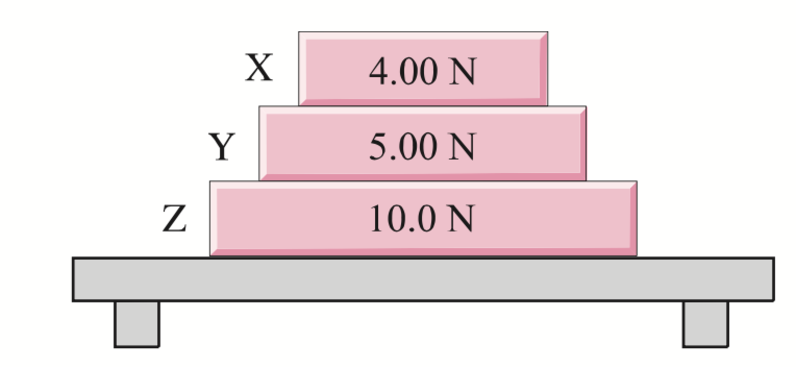
\includegraphics[scale=0.6]{Qfig5-1.pdf}  
  \caption{문제 1}
  \label{fig:1}
\end{figure}
\newpage

{\color{gray} [문제 풀이 쪽]}

\newpage 

\noindent {\bf 문제 2 [10pt]}
화물이 실린 어떤 비행기의 무게는 $2.75\times
10^6$ N이다. 이 비행기의 엔진 추진력이 $6.35\times10^6$ N이라 면 최저
이륙속력인 285 km/h에 도달하기 위해 필요한 활주로의 길이는 최소
얼마인가?  
\newpage

{\color{gray} [문제 풀이 쪽]}

\newpage 

\noindent {\bf 문제 3 [15pt]}
 그림~\ref{fig:3}에서처럼 쓸림이 없는 식탁 위에 레몬이 놓여있다. 이
 레몬에 가해지는, 수평 방향의 힘 세 개 힘 중에서  두 개 $\vec{F}_1$,
 $\vec{F}_2$가 표시되어 있다. 힘 $\vec{F}_1$의 크기는 6.00 N이고,
$\theta_1=30.0^\circ$, $\vec{F}_2$의 크기는 7.00 N,
$\theta_2=30.0^\circ$이다. 
\begin{figure}[ht]
  \centering
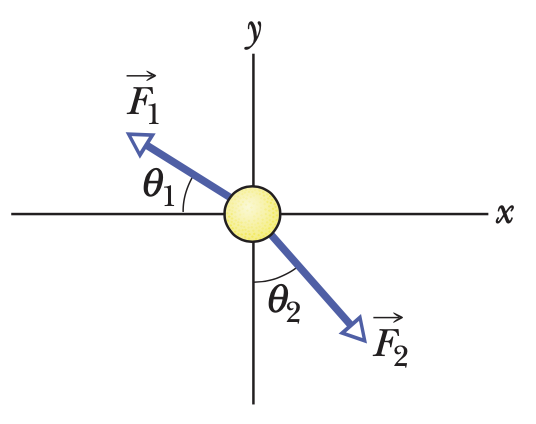
\includegraphics[scale=0.6]{Qfig6-3-20220316.png}  
  \caption{문제 3}
  \label{fig:3}
\end{figure}
\begin{itemize}
\item[(가)] 레몬이 정지해 있으려면,
\item[(나)] 레몬이 일정한 속도 $\vec{v} =(13.0\,\hat{\bm{i}} -
  14.0\,\hat{\bm{j}})\,\mathrm{m/s}$로 움직이려면, 
\item[(다)] 레몬이 속도 $\vec{v} =(13.0t\,\hat{\bm{i}} -
  14.0t\,\hat{\bm{j}})\,\mathrm{m/s}$로 움직이려면, 
\end{itemize}
세 번째 힘은 어떻게 주어져야 하는가? 각각의 경우에 힘을 단위벡터로
표현하여 나타내어라. 
 
\newpage

{\color{gray} [문제 풀이 쪽]}

\newpage

\noindent {\bf 문제 4 [15pt]}
질량이 $1.0\times 10^{-4}$ kg인 공이 줄에 매달려 있다. 수평방향으로
불어오는 일정한 세기의 산들바람이 공을 밀어 줄이 수직과 $45^\circ$를
이루었다.
\begin{itemize}
\item[(가)] 미는 힘의 크기를 구하여라.
\item[(나)] 줄의 장력을 구하여라.
\end{itemize}
\newpage

{\color{gray} [문제 풀이 쪽]}

\newpage
\end{document}